\chapter{Exploration Analytics Methodology}\label{ch3:expl_methods}

\section{Exploration Data Sources}\label{ch3:expl_data_src}

This investigation brings together a total of twenty-five (25) data sets covering the southwest NM study area. Data were collected from previously published works, open-access databases, or derived from those original sources as secondary products. The form of the data varies between pre-gridded raster files, point data sets with repeat or overlapping measurements, non-overlapping point sets, and line data. Previous researchers created raster files or raster-ready gridded data for nine of the features. Four are generated by running procedures on one of the existing rasters. The remaining layers were created from polylines (3), overlapping points (4), and non-overlapping points (2). Although complex interactions between earth systems should be expected, these layers represent the independent variables for analysis purposes. Section XXX details how evaluating collinearities between features allows for pre-screening before modeling, and further analysis of feature importances helps reduce this composite data set to a smaller subset for simpler prediction models.

\begin{table}[htp]
\centering
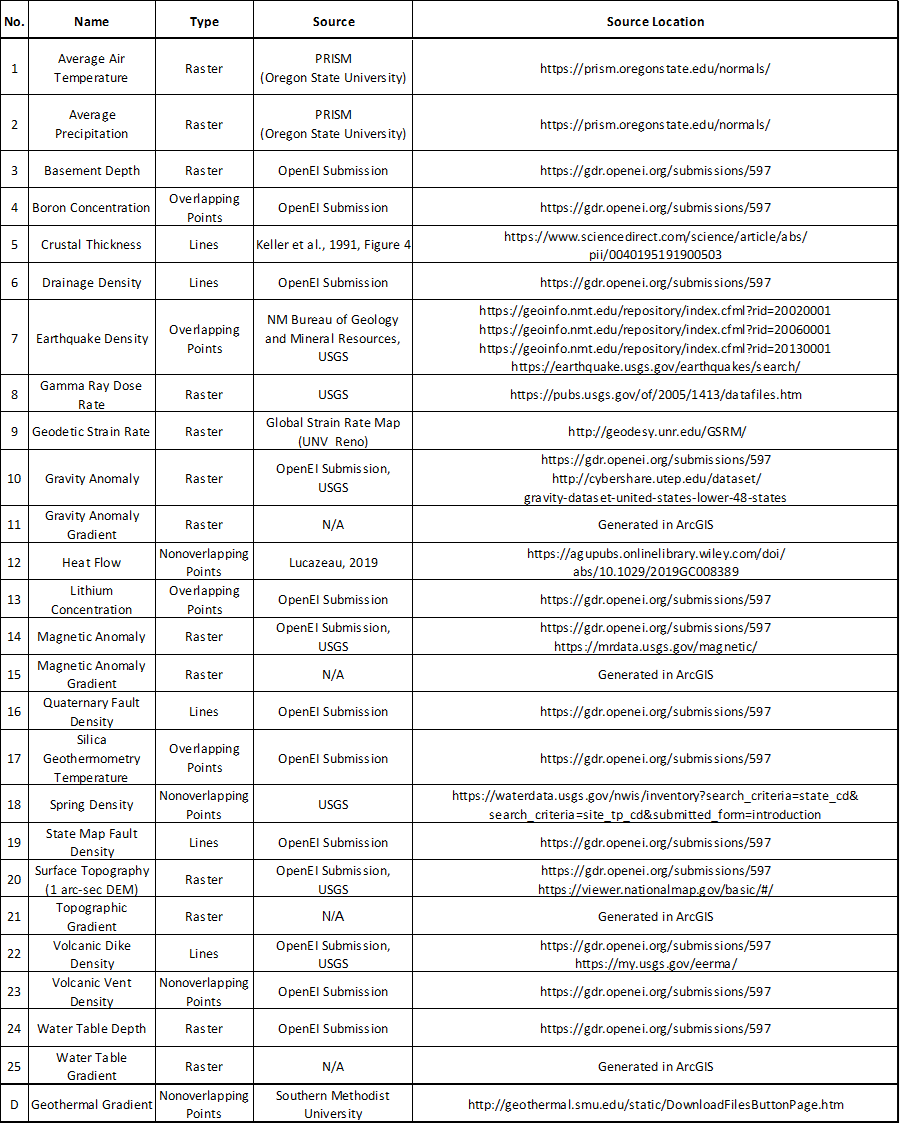
\includegraphics[scale=1]{Table-Features.png}
\caption[Features considered in this the exploration analytics study]{List of data sets considered in this study. Data type, provider, and source location are listed. Numbered features are treated as independent variables. 'D' indicates the dependent variable.}
\label{tab:features}
\end{table}

As discussed in Section \ref{ch2:sysfund}, geothermal systems require permeability, heat, subsurface fluids, a trapping mechanism, and recharge. Following the slightly more simplified PFA assumptions of \citeauthor{bielicki_hydrogeolgic_2015} (\citeyear{bielicki_hydrogeolgic_2015}), an explorationist will want to quickly identify where heat, permeability, and fluids together define a favorable setting for a geothermal prospect. The prepared independent data inputs collectively address all three elements as noted in Table xx. Rather than defining a dependent (predicted) variable that describes a total favorability score, this thesis focuses on a proof of concept prediction for a measurable quantity addressing just the heat risk element: geothermal gradient. This choice was made because a) geothermal gradient provides a direct proxy for accessible heat content, b) gradient point data is available from suitable compilations of well measurements collected across the study area, and c) for EGS applications, the only risk element that must be naturally present is heat. Heat flow might be a reasonable alternative dependent variable, however point values for heat flow in the available well database were derived directly from geothermal gradient values. Geothermometer measurements also suggest resource temperatures, but the uncertainty in fluid pathways leading to the sample location means these values suffer from less spatial and depth certainty than geothermal gradient.

Regarding the remaining two risk elements: direct measurements of permeability (i.e., from downhole logs or core analysis) or fluids (e.g., flow rate from well tests) can be separately predicted using the same methods described in this study. A final favorability score, which is less straight-forward to calibrate for model validation and verification, could potentially be derived from the combined predictions as done in PFA risk assessments. This suggestion is outside of the scope of this thesis and thus appears in the list of future work opportunities (see Chapter 9).

\section{Exploration Data Preparation}

In order to experiment with a variety of machine learning methods, all input data sets first need to be transformed into fully-complete \acrlong{gis} (\acrshort{gis}) layers such that any point on the map of the study area has a corresponding set of 25 independent feature values. Steps taken to condition, process, and otherwise prepare each layer are outlined later in this chapter. As a preface, the following section reviews several key algorithms and concepts applied to one or more of the layers for clarity and reproducibility.

\subsection{Data Preparation Algorithms}

\subsubsection{Extents}

Large data sets imported into ArcGIS or Python for feature preparation required cropping to the southwest New Mexico study area. Two polygons were used for this purpose:

\begin{itemize}
\item Extent Polygon: this is a simple rectangular polygon capturing the broader southwestern NM region. It is defined by the following corner points in degrees N Latitude and degrees E Longitude: \\ (-31.3, -109.1), (31.3, -105.9), (35.4, -105.9), (31.3, -109.1)
\item \acrlong{aoi} (\acrshort{aoi}): this polygon appears in most map figures in this thesis and is the perimeter outlining the nine counties in Southwest New Mexico: Cibola, Valencia, Catron, Socorro, Grant, Sierra, Luna, Dona Ana, and Hidalgo.
\end{itemize}

\subsubsection{Fishnet Points}\label{ssn:fishnet}

\subsubsection{Simple Kriging}\label{ssn:kriging}

\subsubsection{Empirical Bayes Kriging}\label{ssn:ebk}

\subsubsection{Splines}

\subsubsection{Topo to Raster?}

\subsubsection{\acrlong{kde} (\acrshort{kde})}\label{ssn:kde}

\subsection{Data Layers}

\subsubsection{Average Air Temperature}

The University of Oregon PRISM Climate Group hosts regularly-updated spatial data sets of climate-related observations captured from different monitoring networks, including 30-year normals that describe average monthly or annual conditions \citep{daly_physiographically_2008, prism_prism_2021}. 800 m or 4 km resolution grids can be accessed directly from the website. The 800 m resolution air temperature grid was downloaded and imported into ArcGIS, then cropped using the Extent Polygon (Figure \ref{fig:feat_airtemp}). The layer required no further processing.

\begin{figure}[!htp]
\centering
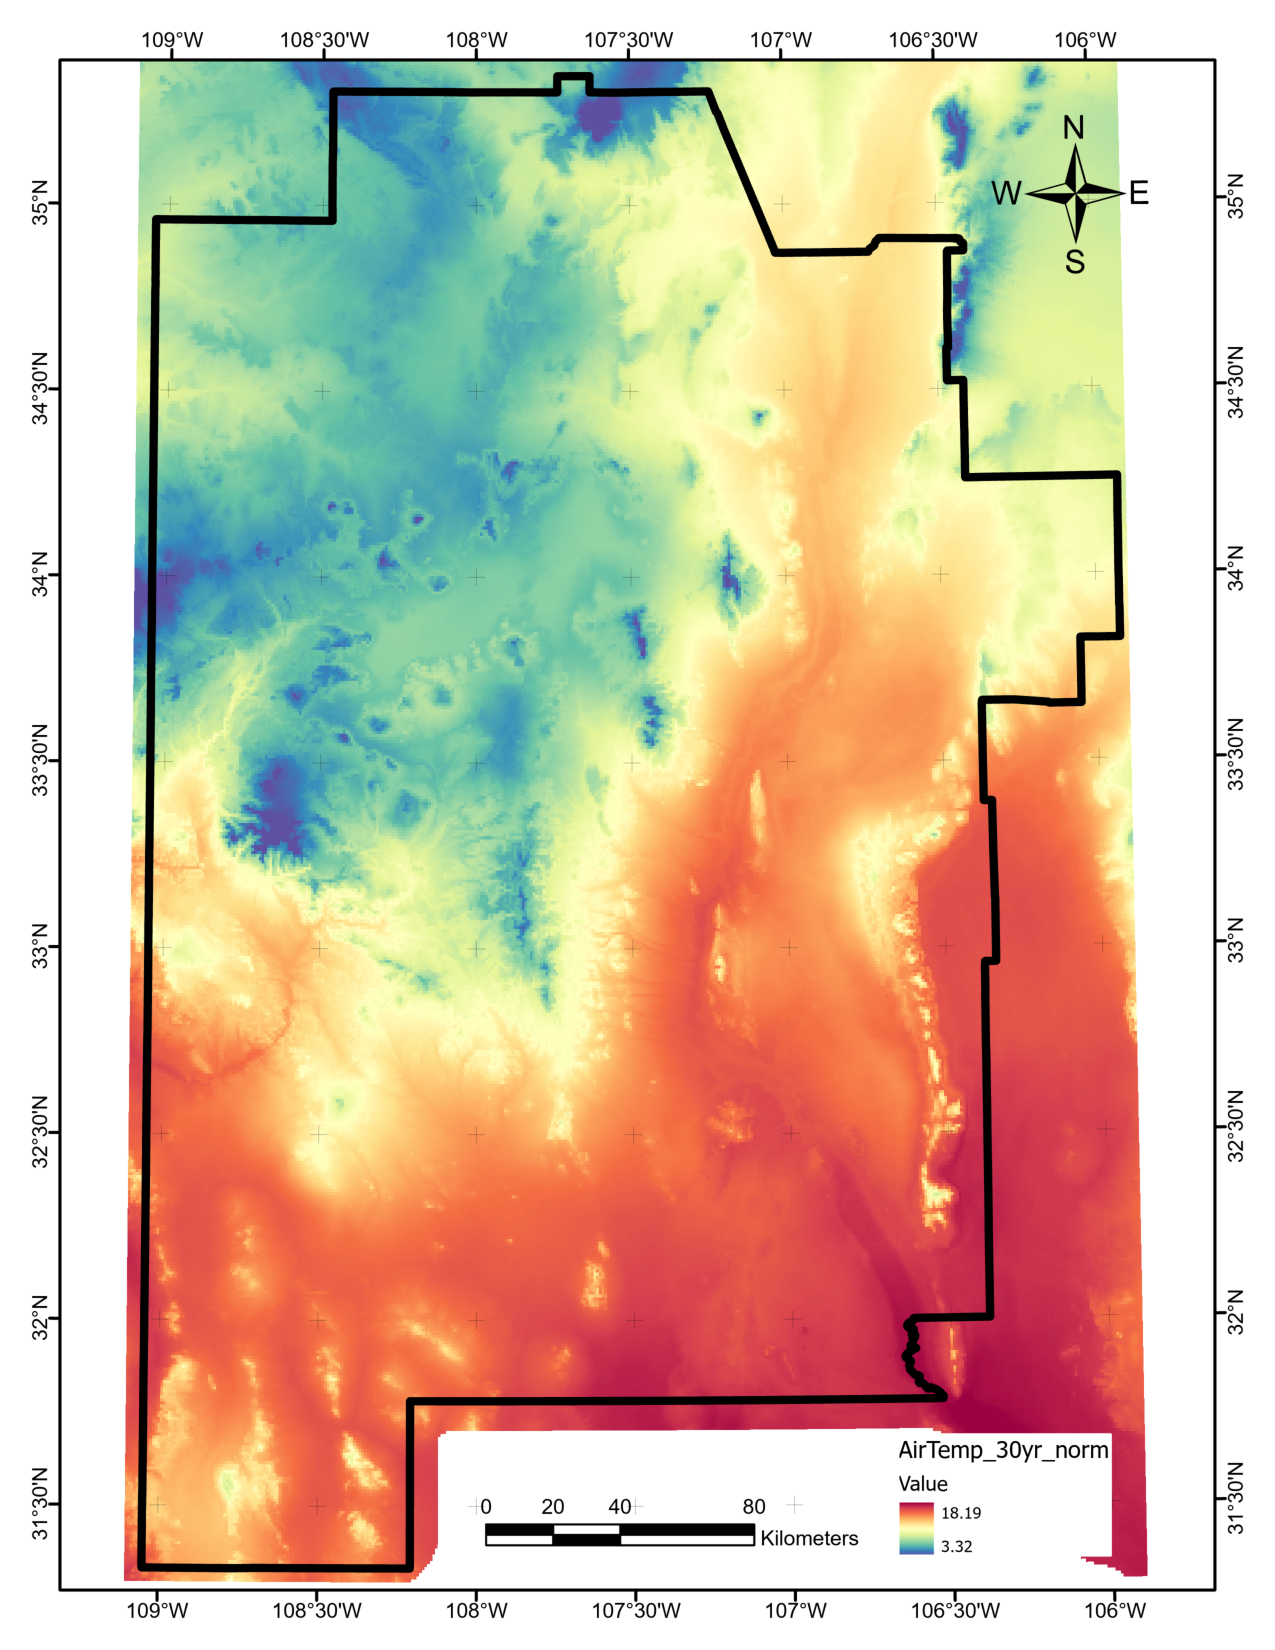
\includegraphics[scale=.6]{Figure-AvgAirTemp}
\caption[Average air temperature data layer]{Average air temperature data layer. Units are degrees Celsius. Data retrieved from \protect\citep{prism_prism_2021}.}
\label{fig:feat_airtemp}
\end{figure}

\subsubsection{Average Precipitation}

The University of Oregon PRISM Climate Group also compiles 30-year normals for average precipitation \citep{daly_physiographically_2008, prism_prism_2021}. The 800 m resolution precipitation grid was downloaded and imported into ArcGIS, then cropped to the Extent Polygon boundaries (Figure \ref{fig:feat_precip}). The layer required no further processing.

\begin{figure}[!htp]
\centering
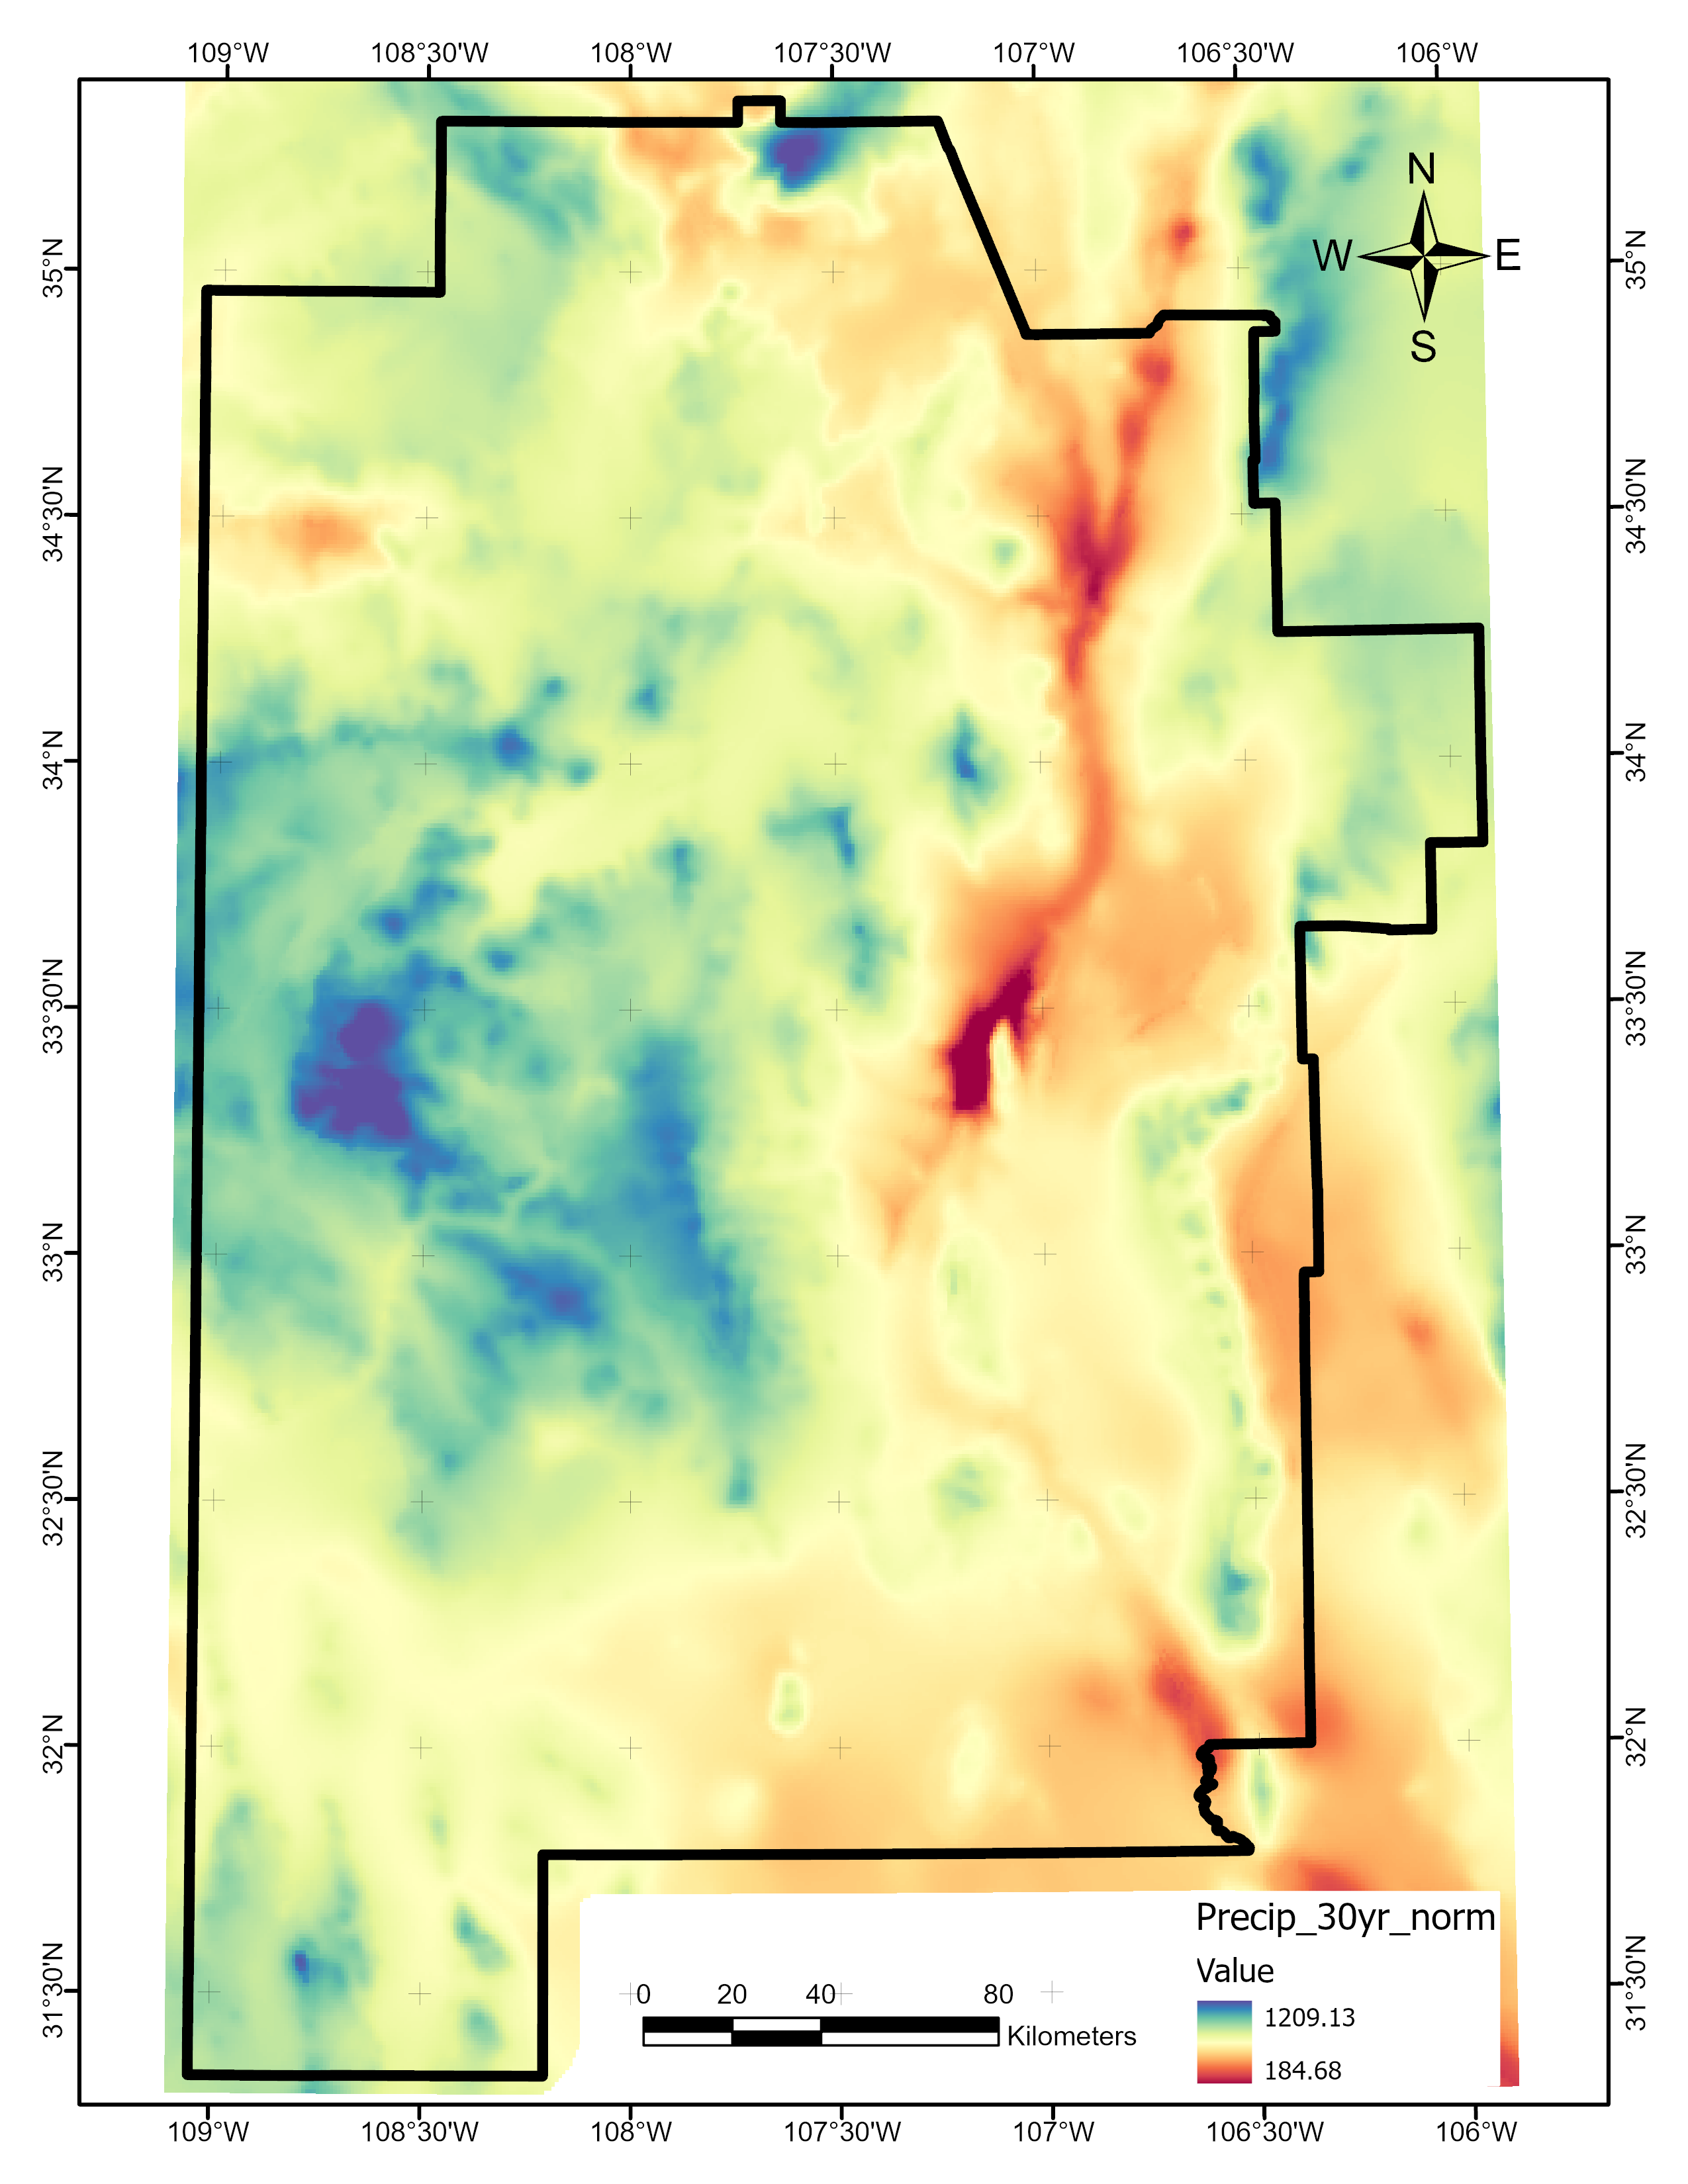
\includegraphics[scale=.6]{Figure-AvgPrecip}
\caption[Average precipitation data layer]{Average precipitation data layer in 800 m resolution. Units are millimeters. Data retrieved from \protect\citep{prism_prism_2021}.}
\label{fig:feat_precip}
\end{figure}

\subsubsection{Basement Depth}

Following the procedure of \citeauthor{pepin_new_2018} (\citeyear{pepin_new_2018}), the basement elevation raster generated by \citeauthor{bielicki_hydrogeolgic_2015} (\citeyear{bielicki_hydrogeolgic_2015}) was downloaded, imported into ArcGIS, and processed to calculate depths. Specifically, a unit conversion from feet to meters was applied. Then, values were extracted on the point fishnet (see \ref{ssn:fishnet}), which highlighted missing data patches in the data. The ArcGIS \textit{Kriging} function interpolated values across these patches using the Ordinary method with Spherical semivariogram, a lag size of 0.096969 automatically determined by ArcGIS, and a variable search radius with a 4-point requirement. Basement depths were then calculated by subtracting the interpolated elevation layer from the surface topography (DEM) layer. However, the higher resolution of the DEM layer caused an imprint of detailed surface geomorphologies to appear on the calculated basement depth layer. To correct for this, the DEM layer was low pass filtered using the ArcGIS \textit{Filter} method, which averages a 3x3 neighborhood around each point in the data set. The final basement elevation layer (Figugre \ref{fig:feat_basementdepth}) was generated from the difference between the low-pass filtered DEM and the kriged basement depth.

\begin{figure}[h!]
\centering
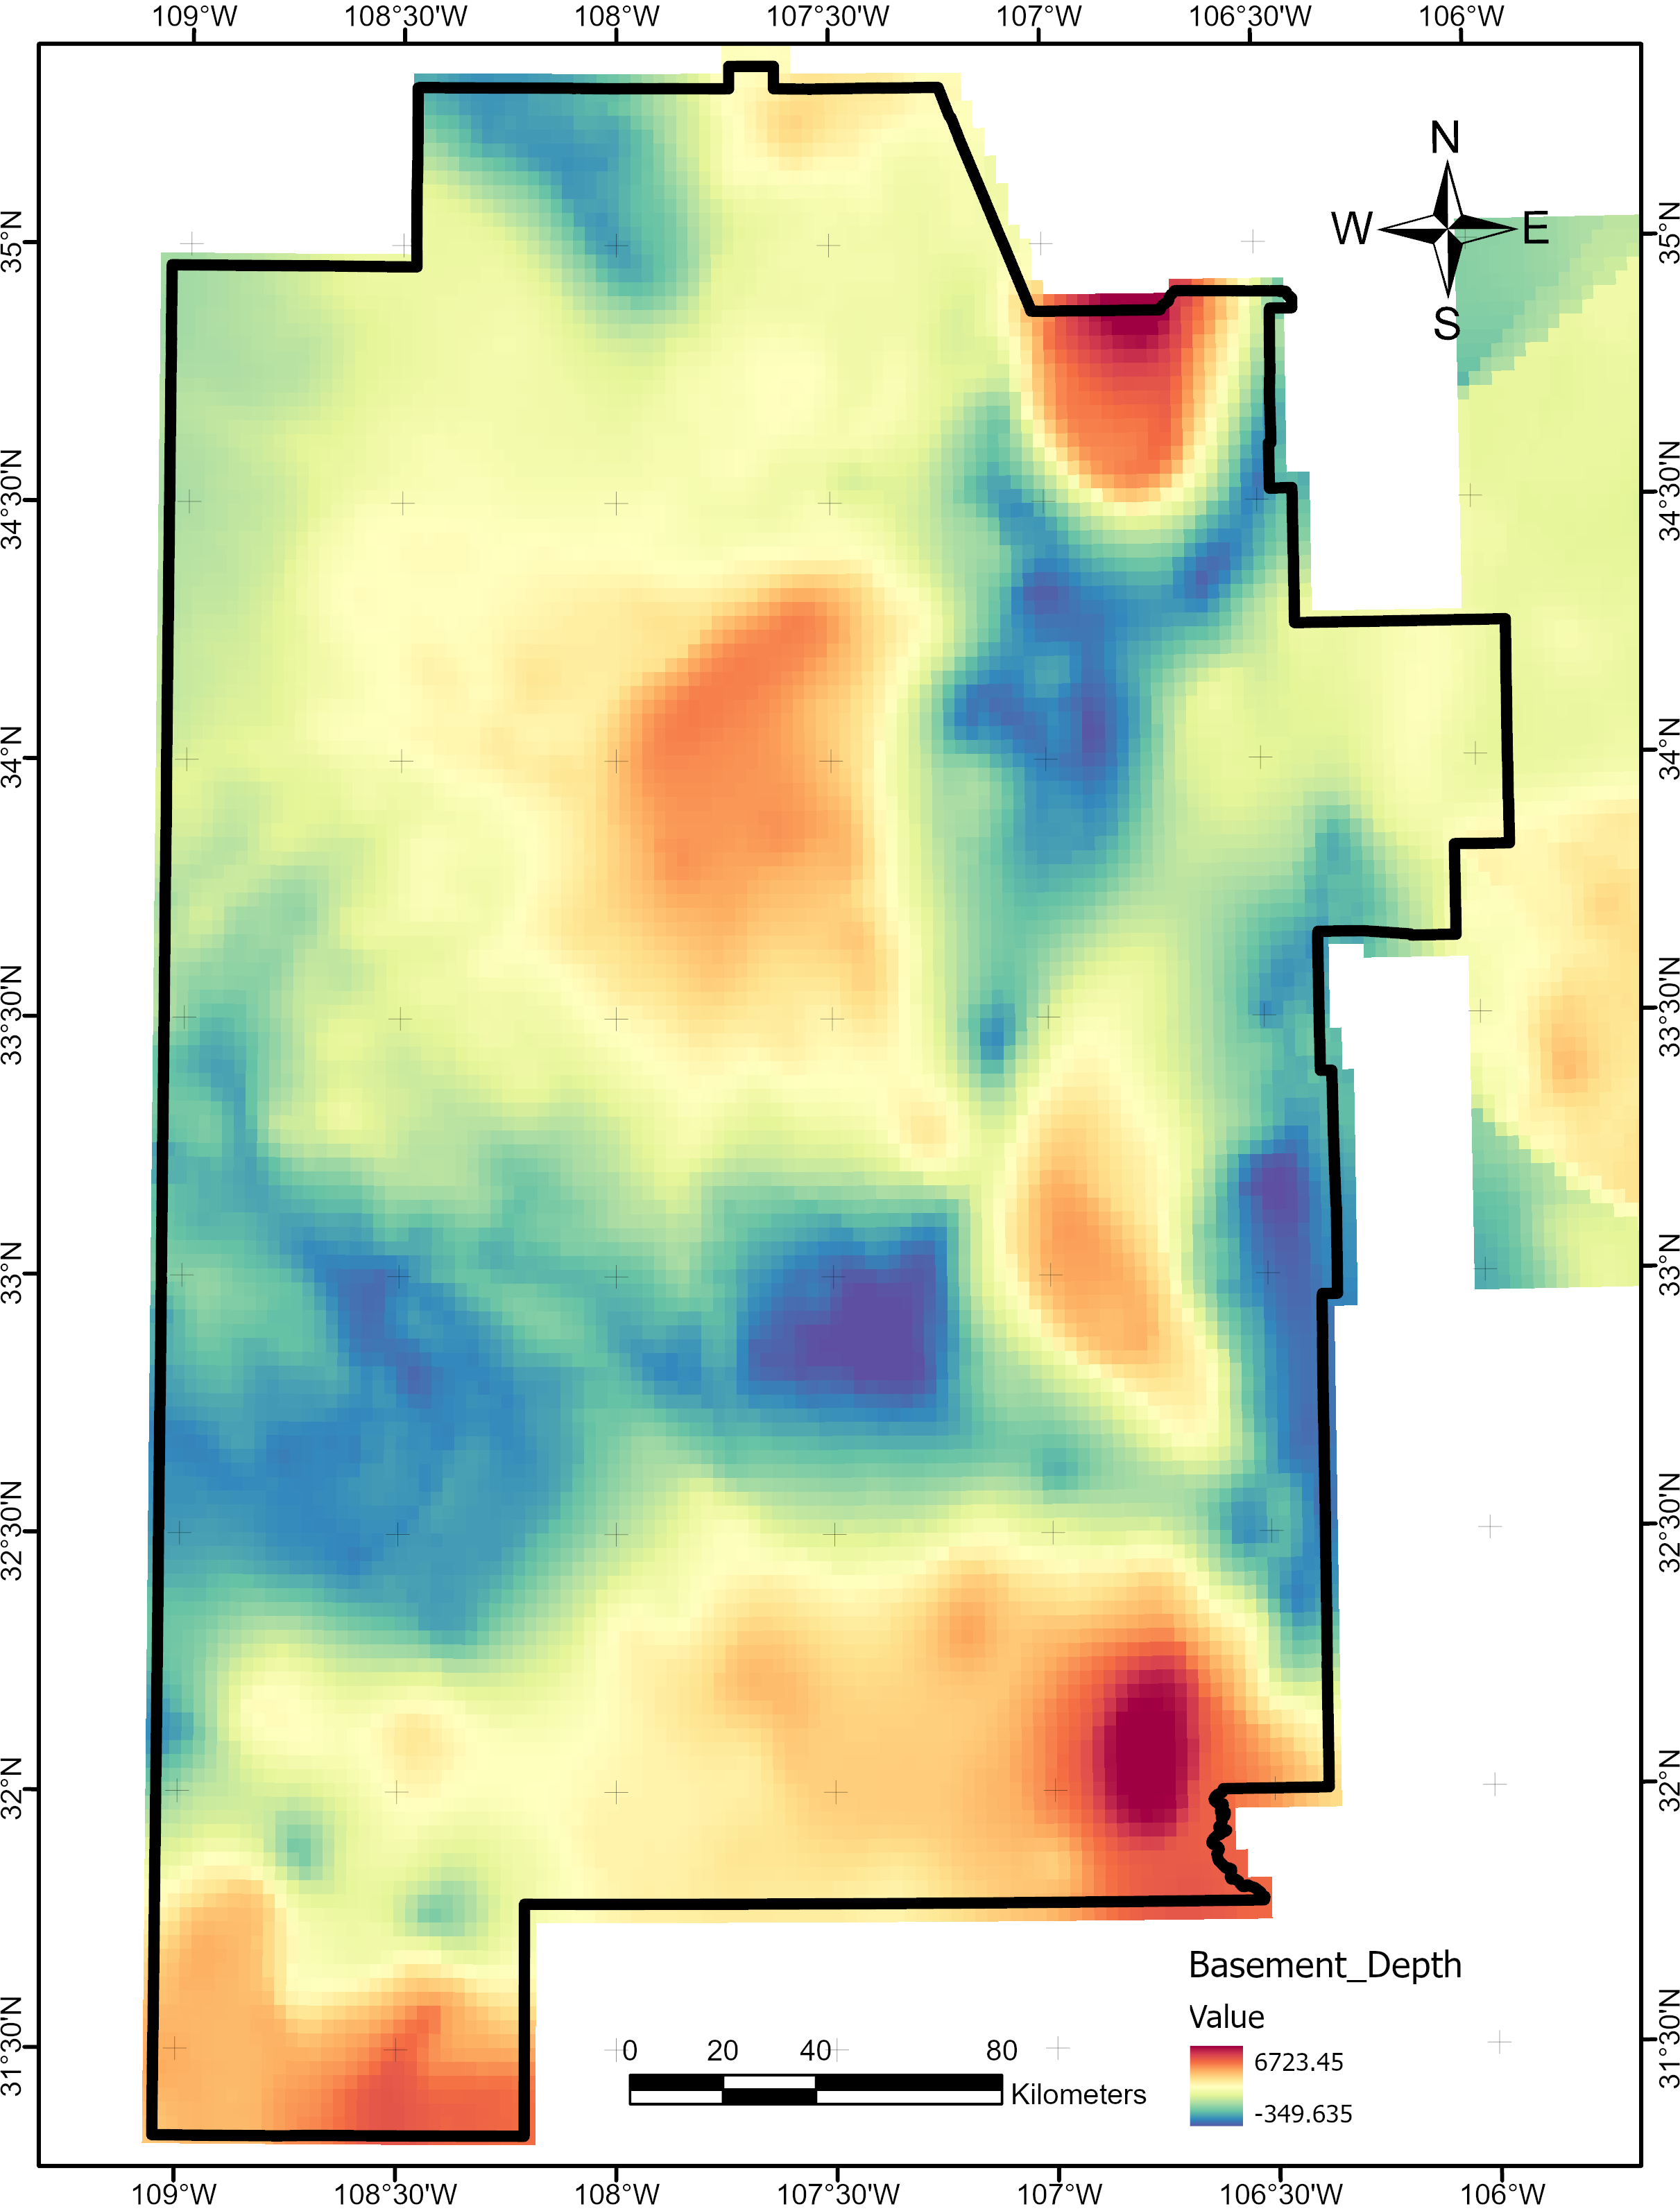
\includegraphics[scale=.6]{Figure-BasementDepth}
\caption[Basement depth data layer]{Basement depth data layer. Units are meters. Layer based on basement elevation raster from \protect\citep{bielicki_hydrogeolgic_2015}.}
\label{fig:feat_basementdepth}
\end{figure}

\subsubsection{Boron Concentration}

Measurements of boron concentration were originally assembled by \citeauthor{bielicki_hydrogeolgic_2015} (\citeyear{bielicki_hydrogeolgic_2015}) from nine sources ranging from USGS records to student dissertations. These data were downloaded from the OpenEI submission \citep{kelley_geothermal_2015} and imported into ArcGIS, then merged into a single dataframe of 5686 measurements within the broader Extent Polygon bounds to avoid edge effects within the AOI. The inconsistent spatial distribution of the data and sometimes significant variation among overlapping values from different measurement years created a unique challenge for making a representative GIS layer to use for analysis. An initial attempt to fit and interpolate the data using tuned Gaussian Process models created feature layers with too much local structure and little character away from the input data points. The ArcGIS \textit{Empirical Bayes Kriging} routine was selected instead due to its unique characteristics. For the final layer (Figure \ref{fig:feat_boron}), EBK was applied with the Empirical data transformation type, a maximum of 100 points in each local model, 100 simulated semivariograms with K-Bessel model type, and a standard circular search neighborhood with a radius of 1.1957 (auto-generated), minimum of 10 neighbors, and maximum of 15 neighbors. The output grid cell size was set to 0.01 degrees. Of important note: the calculation option to include all coincident data was selected, so all overlapping measurements were considered in generating the final layer.

\begin{figure}[h!]
\centering
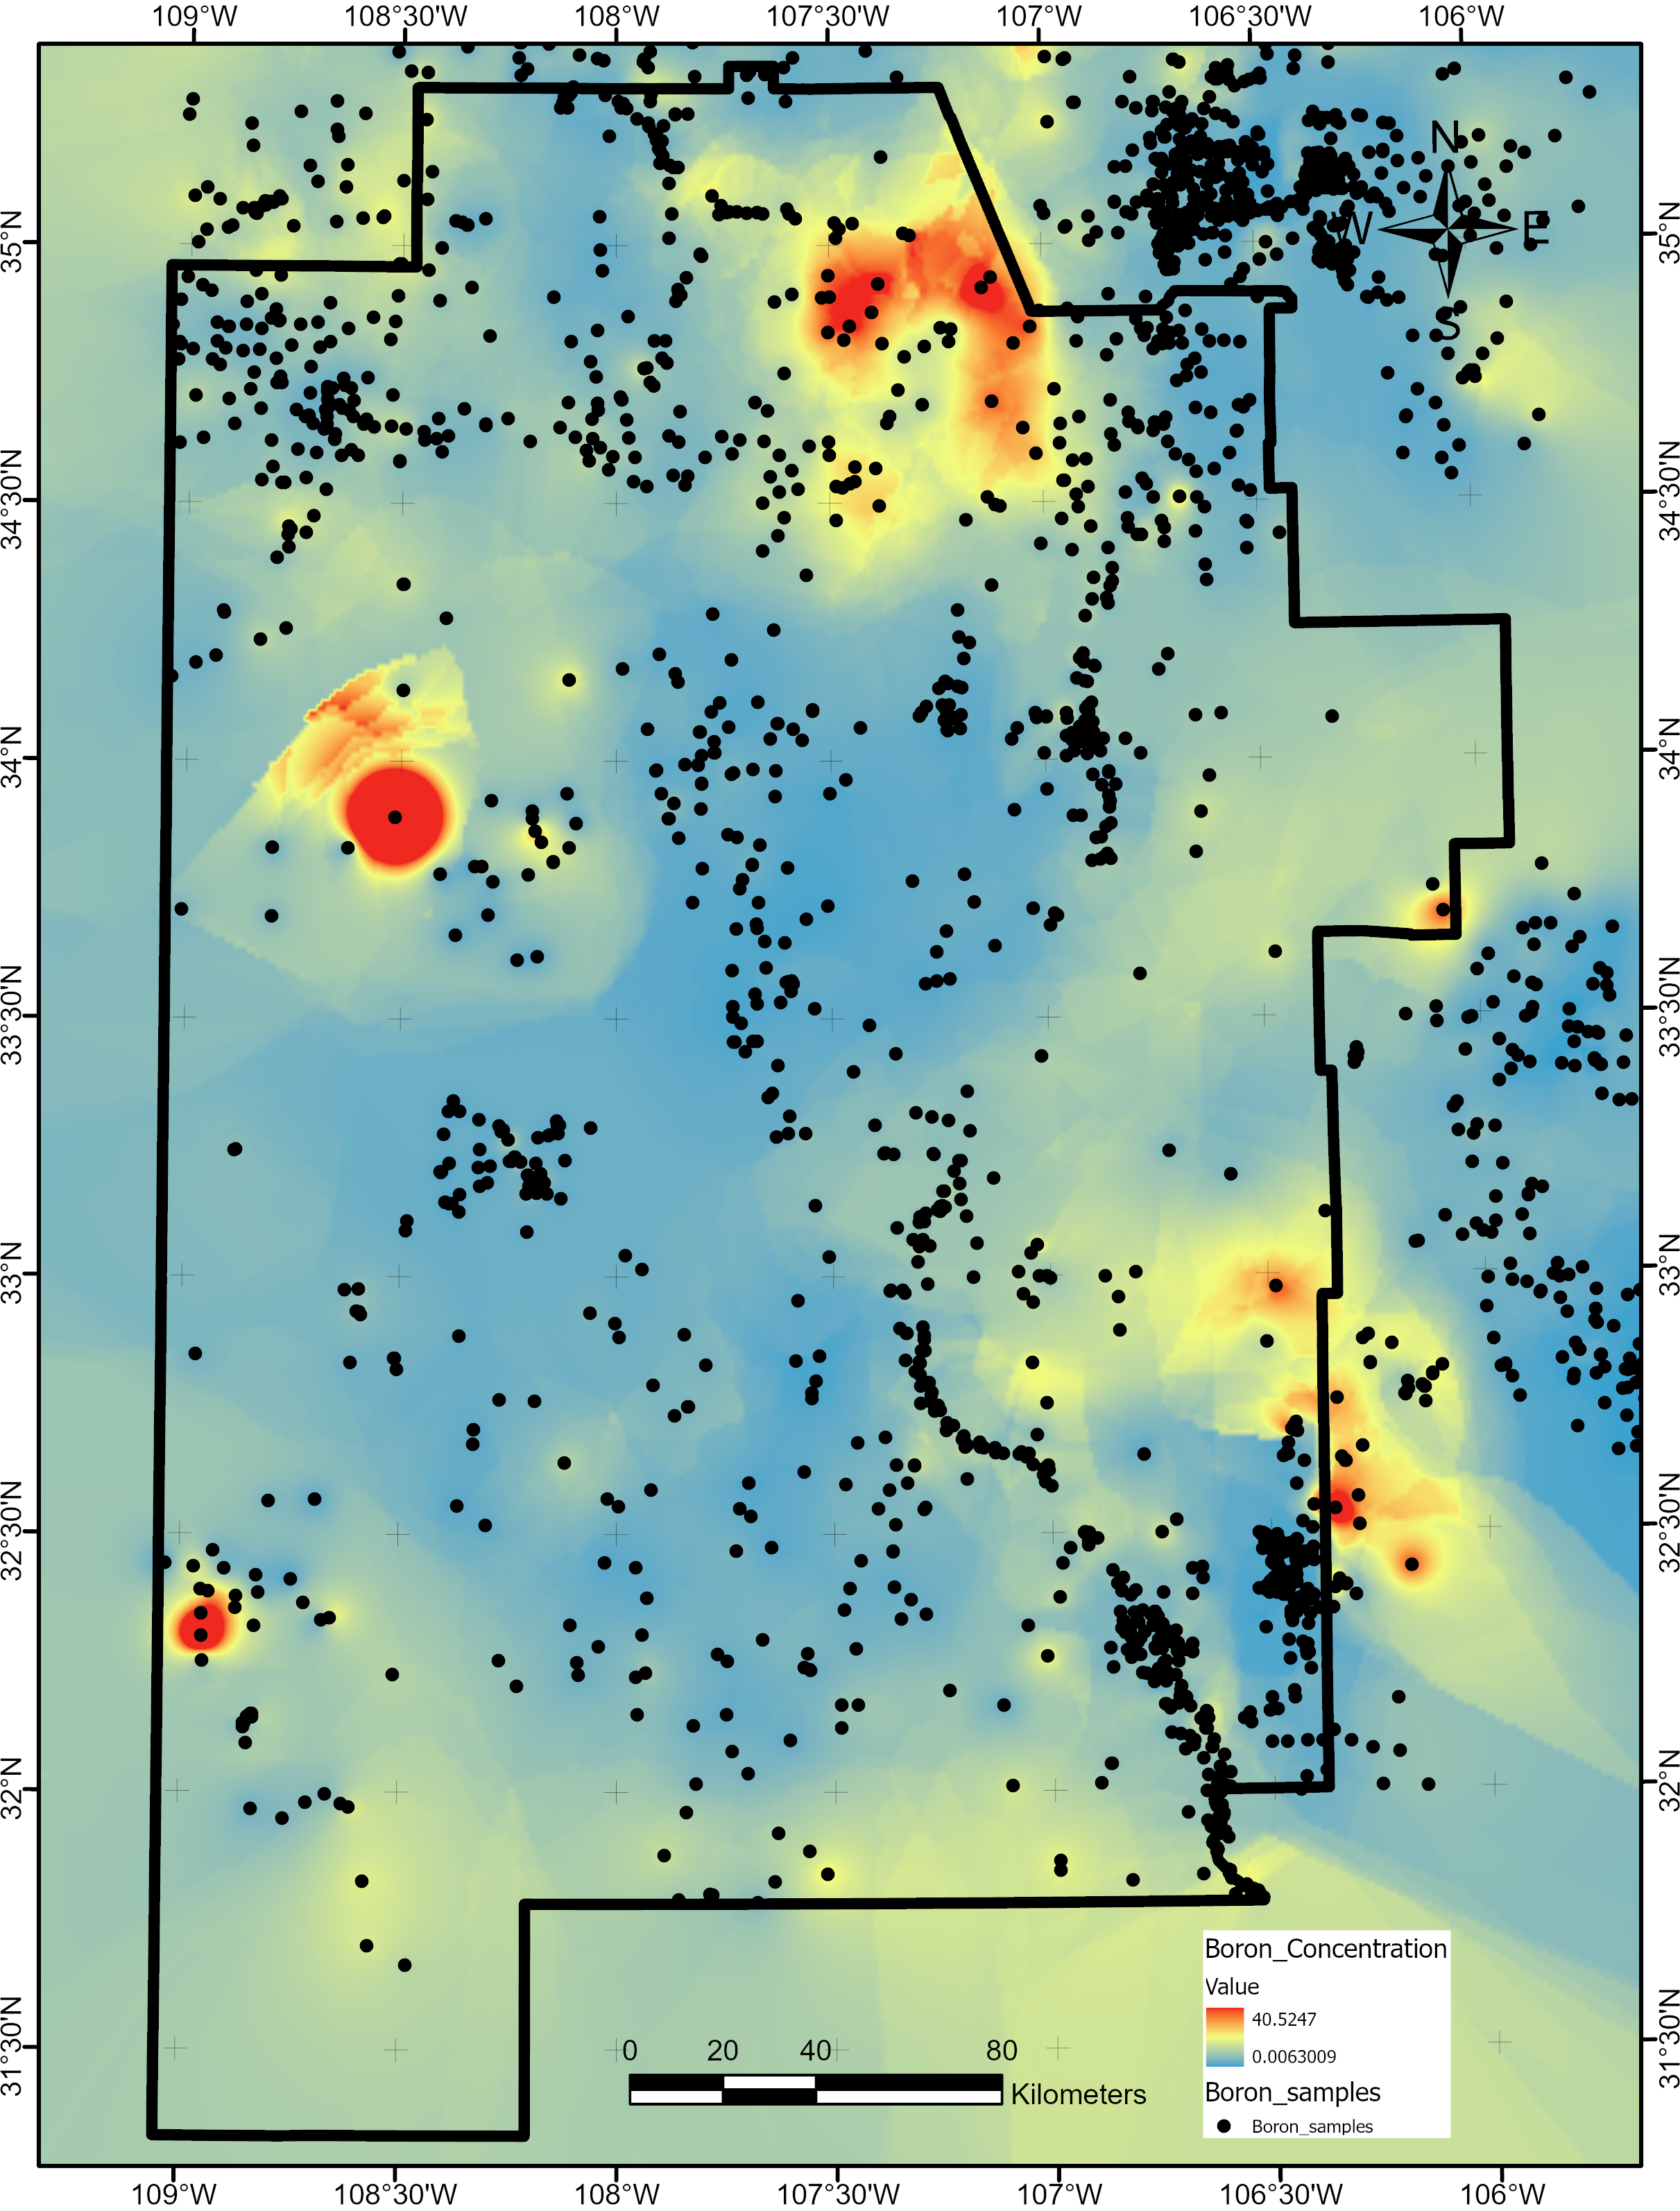
\includegraphics[scale=.6]{Figure-Boron}
\caption[Boron concentration data layer]{Boron concentration data layer. Units in ppm or mg/L. Black dots indicate sample locations in complete data set from \protect\citep{bielicki_hydrogeolgic_2015}.}
\label{fig:feat_boron}
\end{figure}

\subsubsection{Crustal Thickness}

In the absence of a recent 3D seismic survey constraining crustal thickness in the study area, the 2.5D regional map published by \citeauthor{keller_comparative_1991} (\citeyear{keller_comparative_1991}) was used for the crustal thickness feature layer. Similar to the procedure described in \citep{pepin_new_2018}, the Keller map was georeferenced in ArcGIS, and thickness contours were manually digitized as polylines. These polylines continued slightly beyond the AOI boundary to ensure proper constraints for surface creation without artifacts near the AOI edges. The ArcGIS function \textit{Feature to 3D by Attribute} converted the polylines into 3D contours, and \textit{Topo to Raster} generated a continuous final grid (Figure \ref{fig:feat_crust}). Since the Keller map was derived from low-resolution seismic lines from the 1960s-1980s, the result is a very low frequency approximation for crustal thickness variations associated with the CP and RGR. As such, \textit{Topo to Raster} used an output cell size of 0.025 degrees. Other parameters include: margin in the cells of 20, smallest z value for interpolation of 25, largest z value for the interpolation of 55, Enforce selection for drainage enforcement, and maximum iterations of 20.

\begin{figure}[!htp]
\centering
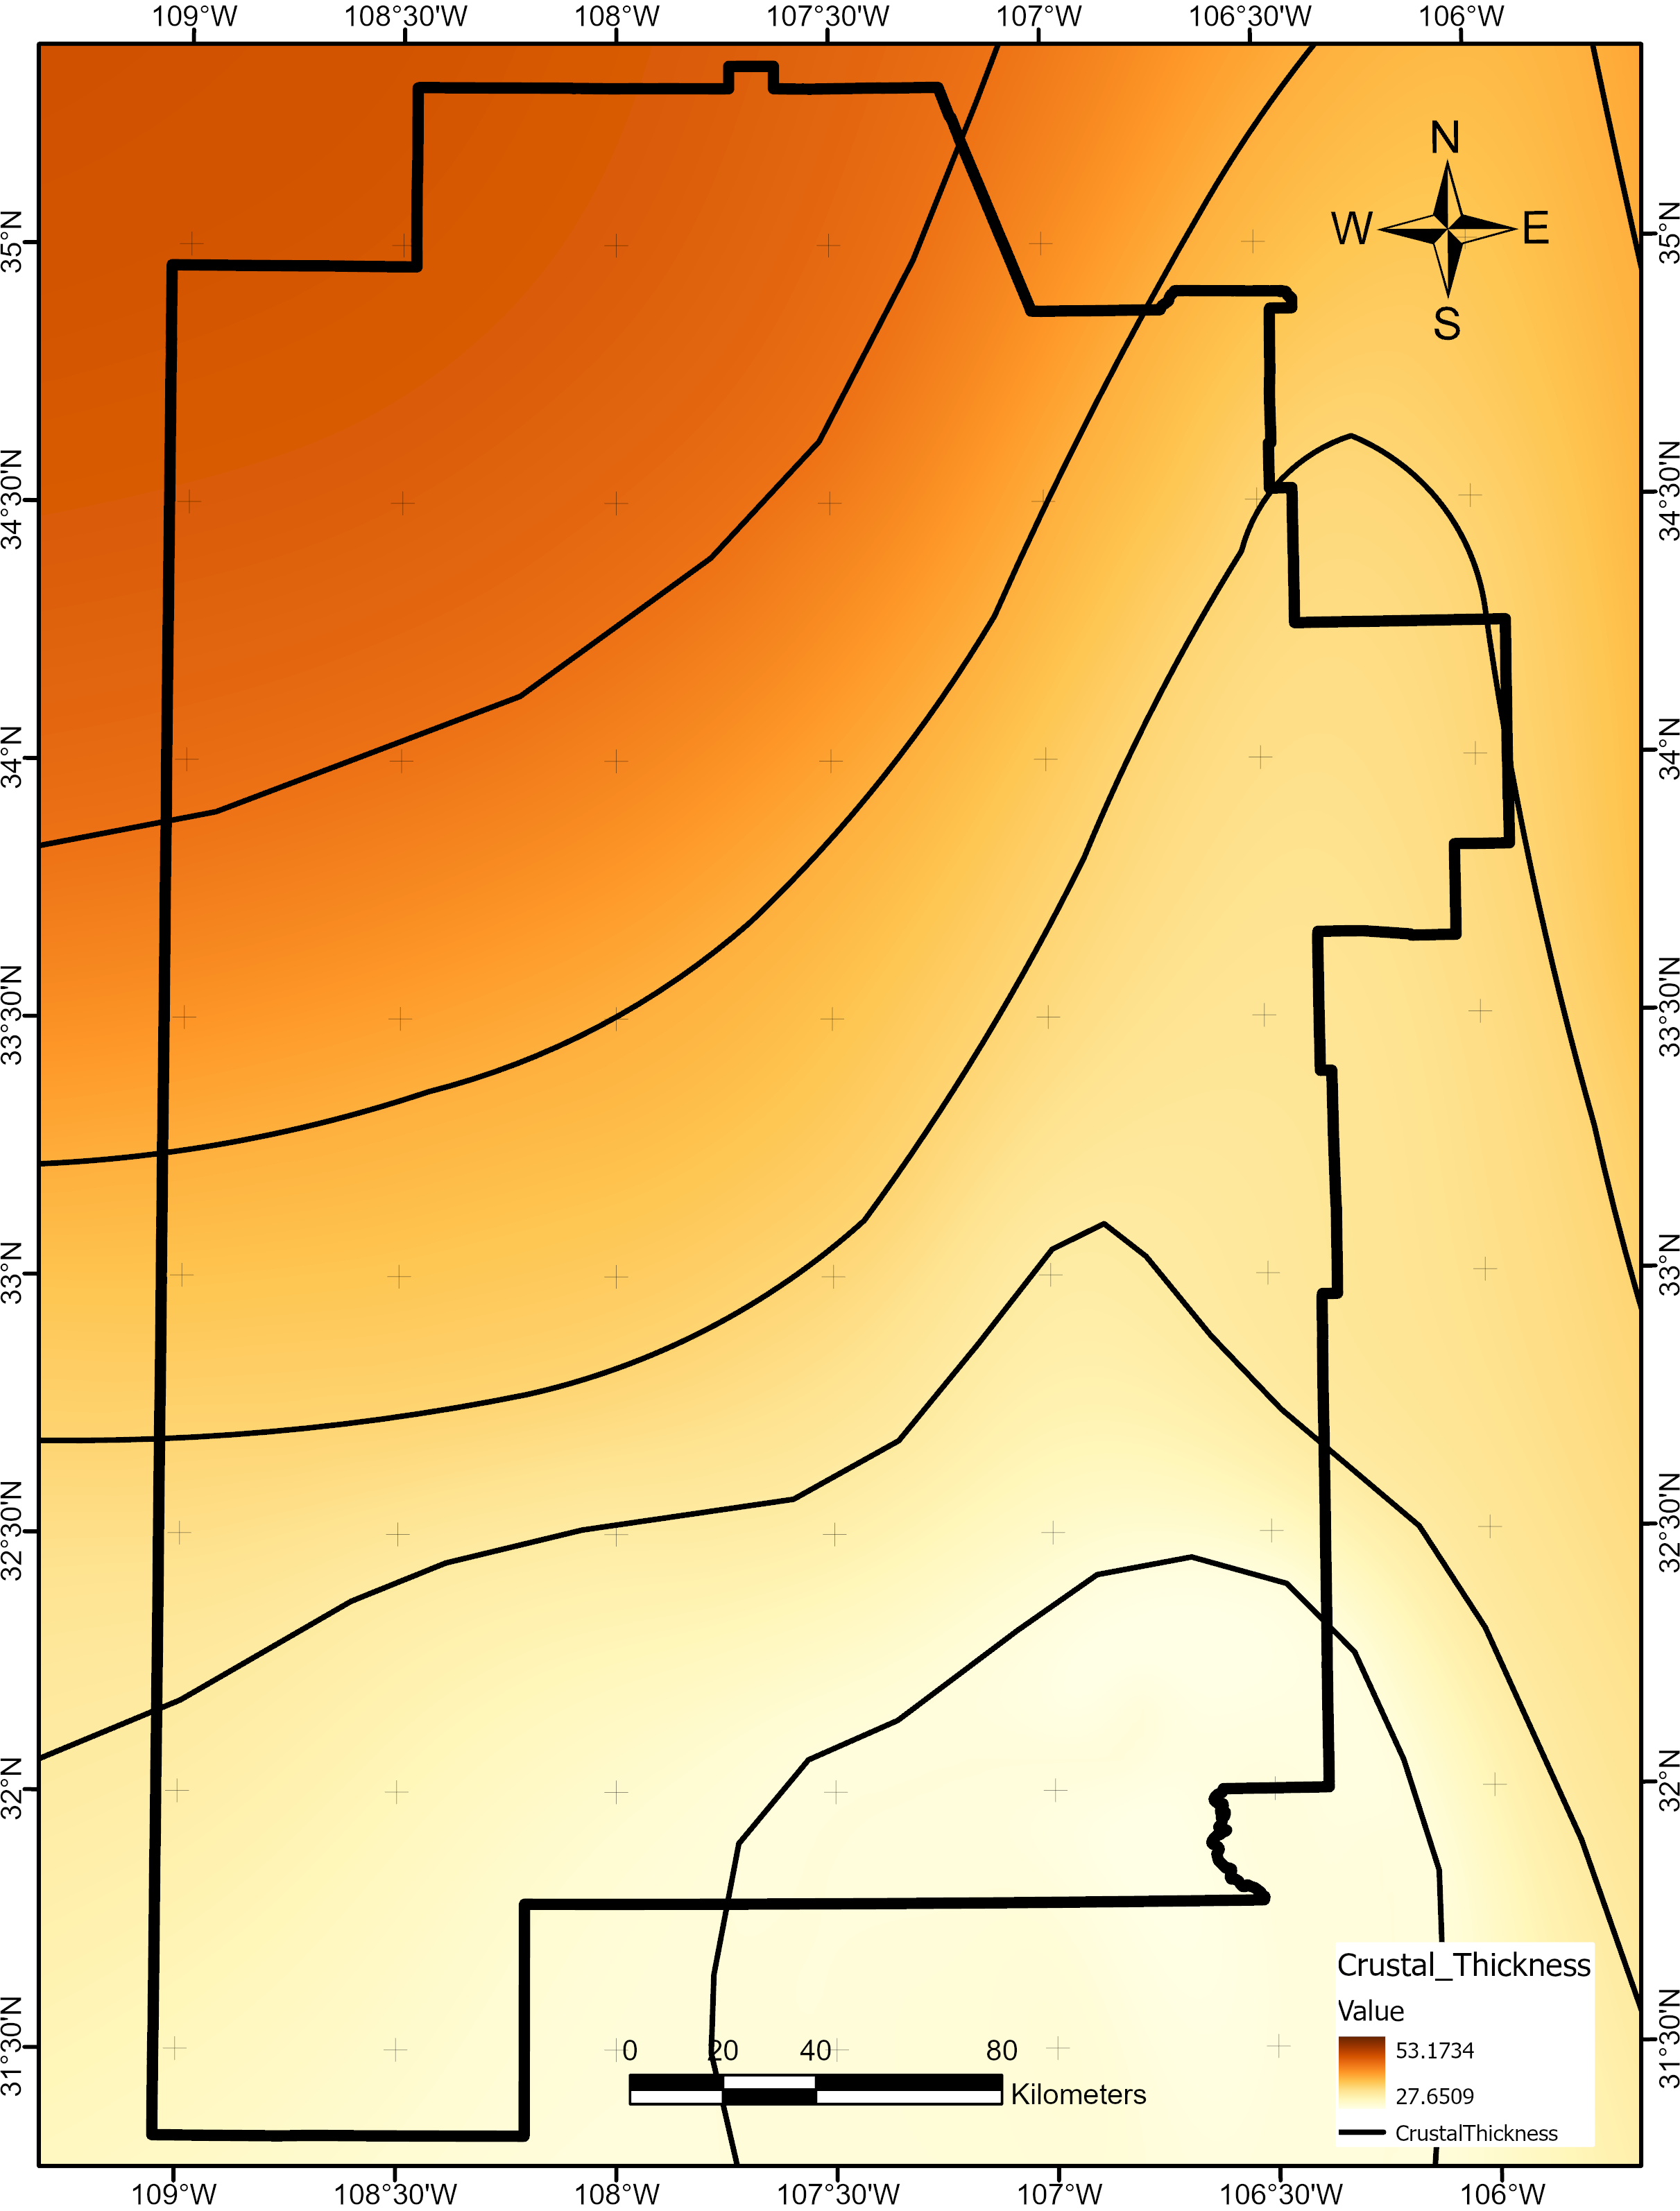
\includegraphics[scale=.6]{Figure-CrustalThickness}
\caption[Crustal thickness data layer]{Crustal thickness data layer. Units in kilometers. Black lines refer to contours digitized from \protect\citep{keller_comparative_1991}.}
\label{fig:feat_crust}
\end{figure}
